\chapter{Anexos} \label{Anexos}

\section{Anexo 1. Estimación de la función de transferencia}\label{ftrans}

	Este anexo está dividido en 2 partes: la primera parte incluye toda la información sobre el proceso de estimación de la función de transferencia descrito en el apartado \ref{subsec:caract_planta} y la segunda parte incluye el script de matlab elaborado para hacer este proceso.

\subsection{Proceso de estimación de la función de transferencia}

	Para estimar la función de transferencia se ha realizado un experimento que consiste en aplicar una señal de entrada escalón de 18{$^{\circ}$}C a 32{$^{\circ}$}C (para cubrir el rango de funcionamiento del sistema de refrigeración) y se ha medido la salida generada por dicho experimento. Este experimento se ha realizado 13 veces durante varios días y a diferentes horas para poder caracterizar mejor el comportamiento dinámico la planta.

	Para cada experimento se ha estimado la función de transferencia que mejor se ajusta a los datos generados en dicho experimento. Se han tenido en cuenta todas las combinaciones posibles de polos y ceros hasta orden 3. La selección de la función de transferencia se ha realizado en base al coeficiente de ajuste. 

	En la tabla \ref{tablaA1.1} se muestra la expresión matemática de la función de transferencia obtenida en cada experimento. Esta tabla sólo incluye la combinación que tiene un mayor coeficiente de ajuste. El resto de combinaciones se han descartado porque es poco probabile que una función que no se ajusta bien a sus propios datos pueda ajustarse mejor a los datos de los otros experimentos.

\newpage 

\begin{longtable}{| c | c | c |}
\hline
\textbf{Num exp} & \textbf{Función estimada} & \textbf{Coef ajuste} \\
\hline 
     &  &   \\
     &  \Large$ G(s) = \frac{6,624 \cdot 10^{-2}s^{2}+ 4,942 \cdot 10^{-4}s + 8,697 \cdot 10^{-7}}{ s^{3} + 0,5169 s^{2} + 3,318 \cdot 10^{-3}s + 1,123 \cdot 10^{-6}} $ &  \\
  1 &  & 91,3831\%  \\
     &  $ z_{1} = -4,6 \cdot 10^{-3},\quad z_{2} = -2,8 \cdot 10^{-3} $ &   \\
     &  $ p_{1} = -0,5104,\quad p_{2} = -6,1 \cdot 10^{-3},$ &  \\
     &  $ p_{3} = -3,583 \cdot 10^{-4}$ &   \\
     &  & \\
\hline
     &  &   \\
     &  \Large$ G(s) = \frac{8,686 \cdot 10^{-2}s+ 1,213 \cdot 10^{-4}}{ s + 1,592\cdot 10^{-4}} $ & \\
  2 &  & 85,5679\% \\
     &  $ z_{1} = -1,4 \cdot 10^{-3} $ &   \\
     &  $ p_{1} = -1.5924\cdot10^{-4} $ &  \\
     &  &   \\
\hline
     &  &   \\
     & \Large $ G(s) = \frac{4.382 \cdot 10^{-3}s+ 4.952\cdot 10^{-6}}{ s^{2} + 0.02972s + 6,397\cdot 10^{-6}} $ &  \\
  3 &  & 89,4146\%  \\
     &  $ z_{1} = -1,1 \cdot 10^{-3} $ &   \\
     &  $ p_{1} = -2,95 \cdot 10^{-2},\quad p_{2} = -2,167 \cdot 10^{-4} $ &  \\
     &  &   \\
\hline
     &  &   \\
     & \Large $ G(s) = \frac{4,976 \cdot 10^{-2}s^{2}+ 1.127 \cdot 10^{-3} + 1,805 \cdot 10^{-6}}{ s^{3} + 0.3519s^{2} + 7,369\cdot 10^{-3} + 2,314 \cdot 10^{-6}} $ \\
  4 &  & 91.4906\%   \\
     &  $ z_{1} = -2,09 \cdot 10^{-2},\quad z_{2} = -1,7 \cdot 10^{-3} $ &   \\
     &  $ p_{1} = -0,3296,\quad p_{2} = -2,20 \cdot 10^{-2},$ &  \\
     &  $ p_{3} = -3,189 \cdot 10^{-4} $ & \\
     &  &   \\
\hline
     &  &   \\
     &  \Large$ G(s) = \frac{2,033 \cdot 10^{-2}s^{2}+ 6.038 \cdot 10^{-4} + 8,775 \cdot 10^{-7}}{ s^{3} + 0.1792s^{2} + 4,498\cdot 10^{-3} + 1.191 \cdot 10^{-6}} $ &  \\
  5 &  & 88.7664\%  \\
     &  $ z_{1} = -2,82 \cdot 10^{-2},\quad z_{2} = -1,5 \cdot 10^{-3} $ &   \\
     &  $ p_{1} = -0,1490,\quad p_{2} = -2,99 \cdot 10^{-2}, $ &  \\
     &  $ p_{3} = -2,6754 \cdot 10^{-4} $ & \\
     &  &   \\
\hline
     &  &   \\
     &  \Large$ G(s) = \frac{8,432 \cdot 10^{-5}s + 1,697 \cdot 10^{-9}}{ s^{3} + 0,282s^{2} + 2,155\cdot 10^{-4} + 1.046 \cdot 10^{-14}} $ &  \\
  6 &  & 90,0349\%  \\
     &  $ z_{1} = -2,0124 \cdot 10^{-5}$ &   \\
     &  $ p_{1} = -0,2813,  p_{2} = -7,663\cdot 10^{-4}, $ &  \\
     &  $ p_{3} = -4,85 \cdot 10^{-11} $ & \\
     &  &   \\
\hline
\newpage
\hline
\textbf{Num exp} & \textbf{Función estimada} & \textbf{Coef ajuste} \\
\hline
     &  &   \\
     &  \large$ G(s) = \frac{8,62\cdot 10^{-10}}{ s^{3} + 1,277 \cdot 10^{-3}s^{2} + 2,333\cdot 10^{-6} + 1.109 \cdot 10^{-9}} $ & \\
  7 &  & 84,4719\%  \\
     &  $ p_{1} = - 3.57\cdot 10^{-4} + 0,0013i,\quad p_{2} = -3.57\cdot 10^{-4}  - 0.0013i, $ &  \\
     &  $ p_{3}=- 5,747 \cdot 10^{-4} $ &   \\
     &  & \\
\hline
     &  &   \\
     &  \large$ G(s) = \frac{7,439 \cdot 10^{-2}s + 1,308 \cdot 10^{-4}}{ s^{2} + 0.5104s^{2} + 1.612\cdot 10^{-4}} $ &  \\
  8 &  & 90,4214\%  \\
     &  $ z_{1} = -1,8 \cdot 10^{-3}$ &   \\
     &  $ p_{1} = -0,5101,\quad p_{2} = -3,1601 \cdot 10^{-4}$ &  \\
     &  &   \\
\hline
     &  &   \\
     &  \large$ G(s) = \frac{7.628 \cdot 10^{-2}s^{2}+ 7.03 \cdot 10^{-4}s + 9.769 \cdot 10^{-7}}{ s^{3} + 0.548s^{2} + 4,787\cdot 10^{-3} + 1.211 \cdot 10^{-6}} $  \\
  9 &  & 91.0543\%  \\
     &  $ z_{1} = -7,5 \cdot 10^{-3},\quad z_{2} = -1,7 \cdot 10^{-3} $ &   \\
     &  $ p_{1} = -0,5392,\quad p_{2} = -8,6 \cdot 10^{-3}, $ & \\
     &  $ p_{3}= -2,61 \cdot 10^{-4} $ &  \\
     &  &   \\
\hline
     &  &   \\
     &  \large$ G(s) = \frac{4,413 \cdot 10^{-7}s + 2,439 \cdot 10^{-9}}{ s^{3} + 8,157 \cdot 10^{-2}s^{2} + 1,603\cdot 10^{-5}s + 3,753 \cdot 10^{-9}} $ &  \\
10 &  & 84,86\%  \\
     &  $ z_{1} = -5,5 \cdot 10^{-3}$ &   \\
     &  $ p_{1} = -8,14 \cdot 10^{-2},\quad p_{2} =-9,825 \cdot 10 ^{-5} + 1,9097 \cdot 10^{-4}i,$ &  \\
     &  $ p_{3} = -9,825 \cdot 10 ^{-5} - 1,9097 \cdot 10^{-4}i, $  &   \\
     &  &  \\
\hline
     &  &   \\
     &  \large$ G(s) = \frac{0,5884s + 1,197 \cdot 10^{-3}}{ s^{3} + 4,457s^{2} + 4,228 s + 1,475 \cdot 10^{-3}} $ &  \\
11 &  & 89,8722\% \\
     &  $ z_{1} = -2,03 \cdot 10^{-3}$ &   \\
     &  $ p_{1} =-3,0877,   p_{2} = -1,3688, $ & \\
     &  $ p_{3} = -3,4898 \cdot 10^{-4} $ &  \\
\hline
     &  &   \\
 12 &  \large$ G(s) = \frac{2,868 \cdot 10^{-4}}{ s + 3,319 \cdot 10^{-4}} \quad p_{1} = -3,3186 \cdot 10^{-4} $ &  89,0861\%\\
     &  &  \\
\hline 
     &  &   \\
     &  \large$ G(s) = \frac{2,449 \cdot 10^{-10}}{ s^{3} + 9,255 \cdot 10^{-3}s^{2} + 4,247 \cdot 10^{-6} s + 2,603 \cdot 10^{-10}} $ & \\
13 &  & 91,05\%  \\
     &  $  p_{1} =-8,8 \cdot 10^{-3},  p_{2} = -4,0788 \cdot 10^{-4}, $ & \\
     &  $  p_{3} = -7,2718 \cdot 10^{-5} $ &  \\
\hline \\
\caption{Tabla con las funciones de transferencia estimadas}\label{tablaA1.1}
\end{longtable}

	Una vez determinada las función de transferencia mejor ajustada en cada experimento, se mide cómo se ajusta cada una de estas funciones a los datos generados por el resto de experimentos. En la tabla \ref{tablaA1.2} se muestra el coeficiente de ajuste de cada función con respecto a sus datos y a los datos de los otros experimentos. Se ha marcado en negro la función que presenta un mejor ajuste para cada experimento.

Analizando los datos de la tabla \ref{tablaA1.2}, se observa que en cada experimento se obtiene un mejor ajuste con los datos propios. El experimento que tiene un mayor coeficiente de ajuste es el número 4 con un valor del 91,4906\%. Sin embargo, puede verse en la tabla que los experimentos 6 y 13 tiene un coeficiente de ajuste medio superior al 80\% y que sus funciones tienen mejores coeficientes de ajuste que el resto. Además, el experimento 6 y el experimento 13 tienen unos coeficientes de ajuste propio de 90,0349\% y 91,05\% respectivamente, luego la variación con el experimento 4 es mínima. Por tanto, se decide que los experimentos 6 y 13 proporcionan una función de transferencia que se ajusta mejor a todos los experimentos. 

	Para decidir cúal de las 2 funciones se aproxima mejor, se va a calcular el error medio y el error máximo absoluto que tienen ambas funciones con respecto a los datos de cada experimento. Además, se van a representar los resultados obtenidos en un diagrama de pareto para visualizarlos mejor. 

	En la tabla \ref{tablaA1.2} puede verse el coeficiente de ajuste, el error cuadrático medio y el máximo error absoluto de ambos experimentos y en las figuras \ref{A1_1:pareto1} y \ref{A1_2:pareto2} se muestra un diagrama de pareto coeficiente de ajuste - error medio y un diagrama de pareto coeficiente de ajuste - error máximo  respectivamente. 

\begin{figure}[H]
  \centering
  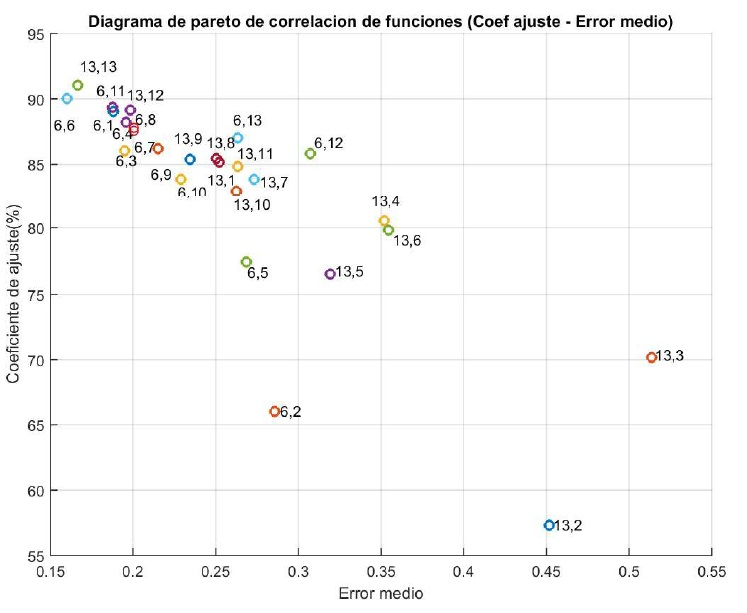
\includegraphics[width=115mm, height=85mm]{imagenes/anexo1/pareto1}
   \caption{Diagrama de pareto coef ajuste - error medio experimentos 6 y 13}
   \label{A1_1:pareto1}
\end{figure}

\begin{figure}[H]
  \centering
  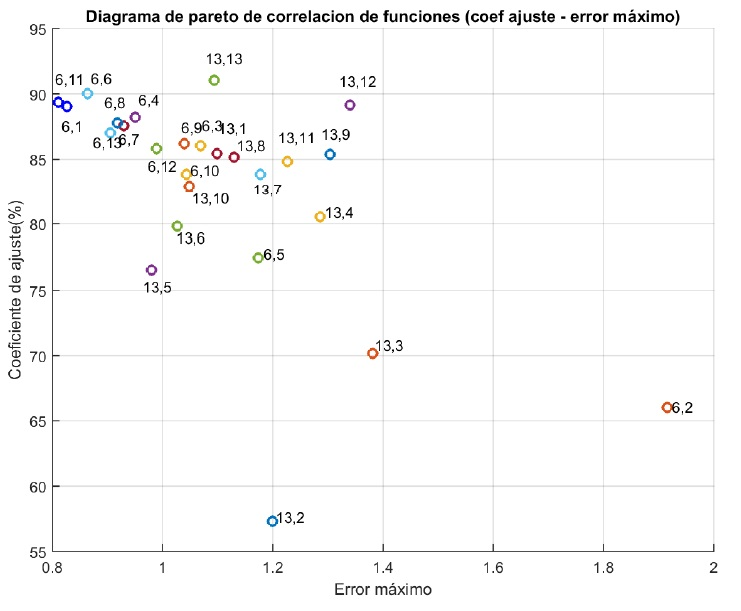
\includegraphics[width=115mm, height=85mm]{imagenes/anexo1/pareto2}
   \caption{Diagrama de pareto coef de ajuste - error máximo experimentos 6 y 13}
   \label{A1_2:pareto2}
\end{figure}

	Examinando dicha tabla se observa que el experimento 6 presenta mejores resultados medios con respecto al experimento 13 en los 3 parámetos. El experimento 6 tiene mejores valores en la mayoría de los experimentos con respecto al experimento 13. En ambos diagramas de pareto se observa que hay un mayor número de casos del experimento 6 situados en la parte superior izquierda de la figura, que se corresponde con un mayor coeficiente de ajuste y un menor error. Por otro lado, se observa que una gran parte de casos del experimento 13 se encuentra en la zona central de la figura, lo que implica que tienen un menor coeficiente de ajuste y un mayor error.

	Por tanto, se concluye que el experimento número 6 proporciona una función de transferencia estimada que se ajusta mejor a los datos de todos los experimentos  que el resto de experimentos y se decide que dicha función es la que mejor caracteriza el comportamiento dinámico de la planta. A continuación se muestra la expresión de dicha función de transferencia:

\begin{equation}\label{ecuacionA1_1}
           G(s) = \frac{8,4315 \cdot 10^{-5}s + 1,6968 \cdot 10^{-9}}{s^{3} + 0,2820s^{2} + 2,1553\cdot 10^{-4}s + 1,0462\cdot10^{-14}}
\end{equation} 

\begin{table}[p]\label{tablaA1.2}
\centering
\begin{sideways}
\scalebox{0.80}[0.90]{
	\begin{tabular}{| c | c | c | c | c | c | c | c | c | c | c | c | c | c | c |}
		\hline
		\multicolumn{15}{|c|}{Coeficiente de ajuste de cada experimento con las funciones estimadas en cada experimento} \\
		\hline
		\textbf{Num Exp} & \textbf{1} & \textbf{2} & \textbf{3} & \textbf{4} & \textbf{5} &\textbf{6} & \textbf{7} & \textbf{8} & \textbf{9} & \textbf{10} & \textbf{11} & \textbf{12} & \textbf{13} & \textbf{Media}\\
		\hline 
			\textbf{1} & \textbf{91,3831} &   7,7316 & 68,1859 & 91,3615 & 41,1466 & 90,1374  & 76,5276  & 74,2446  & 85,5091 &  83,1777 &  69,5568 & 30,6643 &  28,6190  & 62.2385 \\
		\hline
     			\textbf{2} & 46,4539 & \textbf{85,5679} & 63,6155 & 45,7268 & 74,5264 & 45,9584  & 33,6166  & 32,5180  & 40,0218 &  53,1230 &  30,0077 &   5,4745 &    3,0797  & 39,5102 \\
		\hline
			\textbf{3} & 73,0536 & 46,4246 & \textbf{89,4146} & 73,4109 & 77,5897 & 73,0610  & 57,8418  & 56,0292  & 66,0866 &  82,5248 &  52,3741 & 20,8814 &  19,2382  & 58,2096 \\
		\hline
			\textbf{4} & 90,3382 &   4,1194 & 67,5867 & \textbf{91,4906} & 41,9392 & 88,6594  & 76,7551  & 74,3276  & 85,7107 &  82,9944 &  69,6904 & 32,8622 &  31,3778  & 62,1968 \\
		\hline
			\textbf{5}& 58,2029  & 77,8641 & 69,5411 & 53,1426 & \textbf{88,7664} & 52,0389  & 36,8298  & 36,0635  & 43,4967 &  63,5883 &  32,9378 &  -4.4508 &  -9,3537  & 42.4918 \\
		\hline
			\textbf{6} & 89,0111  & 66,0086 & 86,0577 & 88,2092 & 77,4787 & \textbf{90,0349}  & 87,5776  & 87,7922  & 86,2082 &  83,8632 &  89,3537 & 85,8163 &  86,9912  & 84,5306 \\
		\hline
			\textbf{7} & 64,1301  &-29,3008 & 40,0983 & 68,4246 & -1.3793 & 67,5641  & \textbf{84,4719}  & 85,7168  & 75,2369 &  51,2921 &  84,5548 &  41,7830 & 38,3973  & 48,8765 \\
		\hline
			\textbf{8} & 75,5006  &-49,2439 & 33,4329 & 70,8841 & 10,6069& 67,0687  & 89,3440  & \textbf{90,4214}  & 78,5941 &  56,8271  &  88,3031 & 57,9744 & 58,9475  & 53,1866 \\
		\hline
			\textbf{9} & 89,6178  &-14,5296 & 54,8458 & 86,3504 & 39,7781& 83,3306  & 84,2851  & 81,8112  & \textbf{91,0543} &  77,8724  &  77,1474 & 48,0135 & 49,1641  & 63,1406 \\ 
		\hline
			\textbf{10} & 84,6609  & 67,2489 & 71,1708 & 84,5313 & 81,3005& 85,2595  & 84,9659  & 85,4456  & 84,5013  & \textbf{84,8600}   &  84,7497 &  63,8425 & 49,2469  & 77,2436 \\
		\hline
			\textbf{11} & 68,6527  &-60,2874 & 25,9336 & 64,1865 & -0.2220 & 60,4990  &85,8828  & 88,6983  & 72,3367  & 48,8204  &\textbf{89,8722}    & 61,1804  & 61,8088  & 48,1242 \\
		\hline
			\textbf{12} & 43,1090  &-134,0588 & -24,8806 & 26,2330 &-35,0181  & 21,6890 & 52,6691  & 58,4728   &35,7301  & 14,2683 &64,2494 & \textbf{89,0861} & 85,9484 & 17,3676 \\
		\hline
			\textbf{13} & 85,4331  & 57,3050 & 70,1803  & 80,5133 & 76,5364 & 79,8458 & 83,8308  & 85,1552 & 85,3857 & 82,9430 & 84,8552 &89,1679 &       \textbf{91,0500} &  80.0960\\
		\hline
                     \multicolumn{15}{|c|}{} \\
		\multicolumn{15}{|c|}{} \\
                     \hline
		\multicolumn{15}{|c|}{Coeficiente de ajuste de los experimentos 6 y13} \\
		\hline
			\textbf{Num Exp} & \textbf{1} & \textbf{2} & \textbf{3} & \textbf{4} & \textbf{5} &\textbf{6} & \textbf{7} & \textbf{8} & \textbf{9} & \textbf{10} & \textbf{11} & \textbf{12} & \textbf{13} & \textbf{Media}\\
		\hline 
			\textbf{6} & 89,0111  & 66,0086 & 86,0577 & 88,2092 & 77,4787 & \textbf{90,0349}  & 87,5776  & 87,7922  & 86,2082 &  83,8632 &  89,3537 & 85,8163 &  86,9912  & 84,5306 \\
		\hline
			\textbf{13} & 85,4331  & 57,3050 & 70,1803  & 80,5133 & 76,5364 & 79,8458 & 83,8308  & 85,1552 & 85,3857 & 82,9430 & 84,8552 &89,1679 &  \textbf{91,0500} &  80.0960\\
		\hline
			\multicolumn{15}{|c|}{} \\
		\hline 
			\multicolumn{15}{|c|}{Error cuadrático medio de los experimentos 6 y 13} \\
		\hline
			\textbf{Num Exp} & \textbf{1} & \textbf{2} & \textbf{3} & \textbf{4} & \textbf{5} &\textbf{6} & \textbf{7} & \textbf{8} & \textbf{9} & \textbf{10} & \textbf{11} & \textbf{12} & \textbf{13} & \textbf{Media}\\
		\hline 
			\textbf{6} & 0,1881  &  0,2859  &  0,1951  &  0,1956  &  0,2684  & \textbf{0,1599} & 0,2006  & 0,2006   &  0,2150  &  0,2291  &  0,1875   & 0,3074  &  0,2632  & 0,2280 \\
		\hline
			\textbf{13} & 0,2504    & 0,4515   &  0,5135   &  0,3518    & 0,3193  &  0,3546   & 0,2732    & 0,2523   &  0,2347   & 0,2625  & 0,2635  &  0,1985  &\textbf{0,1666} & 0,3105 \\
		\hline
			\multicolumn{15}{|c|}{} \\
		\hline 
			\multicolumn{15}{|c|}{Error máximo de los experimentos 6 y 13} \\
		\hline
		\textbf{Num Exp} & \textbf{1} & \textbf{2} & \textbf{3} & \textbf{4} & \textbf{5} &\textbf{6} & \textbf{7} & \textbf{8} & \textbf{9} & \textbf{10} & \textbf{11} & \textbf{12} & \textbf{13} & \textbf{Media}\\
		\hline 
			\textbf{6}  & 0,8270    & 1,9157    & 1,0695    & 0,9497    & 1,1739  & \textbf{0,8637}    & 0,9297    & 0,9183    & 1,0394    &1,0433   & 0,8114    & 0,9891    & 0,9058    & 1,0477 \\
		\hline
			\textbf{13} & 1,0991    & 1,1993    & 1,3817    & 1,2856    & 0,9804   & 1,0266   & 1,1769    & 1,1300    & 1,3033    & 1,0482   & 1,2258    & 1,3396    & \textbf{1,0941}    & 1,1830  \\
		\hline
\end{tabular}}
\end{sideways}
\caption{Coeficiente de ajuste de cada función con el resto de experimentos}
 \end{table}

\newpage	
\subsection{ Scripts de matlab para hacer la estimación}

	Este apartado incluye los scripts de matlab que se han diseñado para calcular la estimación de la función de transferencia. Se han diseñado 4 scripts.

\begin{itemize}
	\item\textbf{estimador.m:} este script se utiliza para extraer los datos de la plataforma y realizar la estimación de la función de transferencia para todas las combinaciones hasta orden 3.
	\item\textbf{seleccionarEstimacion.m:} este script se utiliza para seleccionar de cada experimento la función de transferencia que tiene un mejor coeficiente de ajuste.
	\item\textbf{analizador.m:} este script se utiliza para realizar la correlación entre todas las funciones de transferencia de todos los experimentos y seleccionar la función de transferencia que mejor se aproxima a todos los experimentos.
	\item\textbf{conv\_hora\_unix.m:} función que se utiliza para convertir la hora a formato unix. Esta función se utiliza en el script estimador.m.
\end{itemize}

	Para mayor claridad y debido a la longitud de estos scripts, se ha decidido no incluir el código en esta memoria. En su lugar, se ha habilitado un repositorio en github donde se pueden consultar estos scripts. La dirección http de este repositorio es la siguiente: \textbf{https://github.com/jccalvo/TFG.git}


 \newpage
    


